% Resultados: presenta tablas/figuras y comenta hallazgos clave.

%\subsection{Ejemplo de figura} % Sub-sección para ilustrar resultados gráficos
% \begin{figure}[!t]             % Entorno de figura; [!t]=arriba, con preferencia fuerte (!)
 %  \centering
  % includegraphics: inserta imagen externa
  % keepaspectratio: conserva la relación de aspecto al escalar
  % width=0.9\linewidth: ancho al 90% de la línea actual (se puede usar height=...)
%   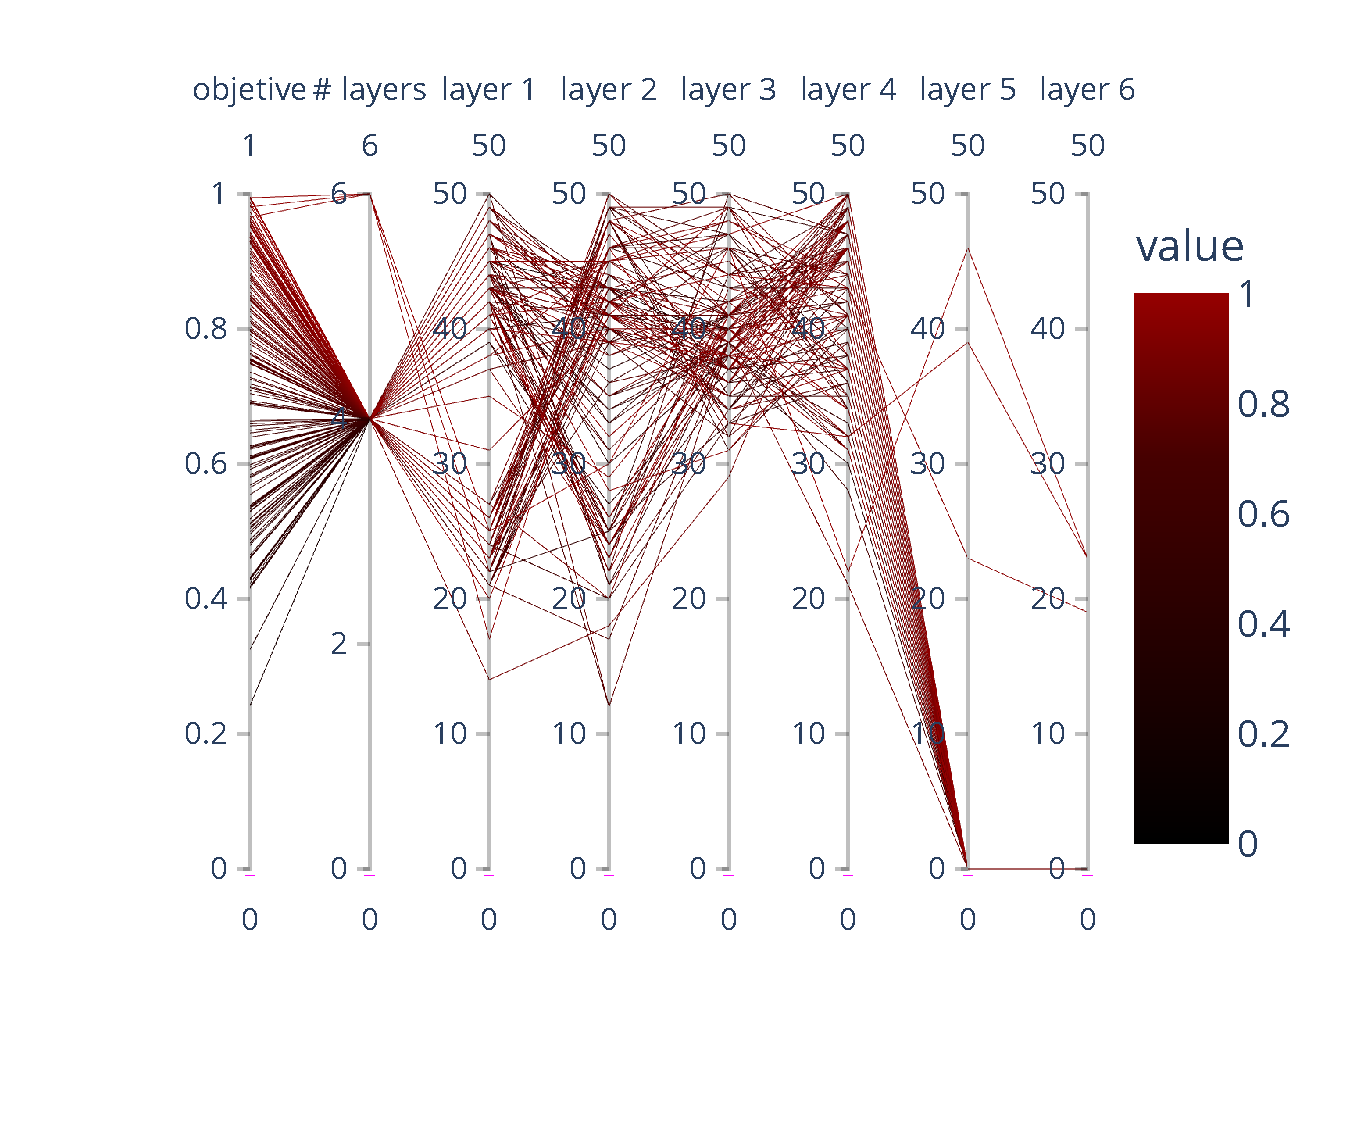
\includegraphics[keepaspectratio, width=0.9\linewidth]{images/neurons.pdf}
%   \caption{Figura de ejemplo generada con PGF (sustituible por tus resultados).} % Texto bajo la figura
%   \label{fig:res_fig}          % Etiqueta para referenciar con \ref{fig:res_fig}
% \end{figure}

%\subsection{Ejemplo de tabla}  % Sub-sección para resultados en formato tabla
 % \input{tables/table2.tex}      % Inserta archivo de tabla externa en este punto

% Consejos: Compara contra una línea base y reporta métricas con su interpretación.